\documentclass[12pt]{beamer}
\usepackage{xcolor}
\usepackage{pgf,pgfarrows,pgfnodes,pgfautomata,pgfheaps,pgfshade}
\usepackage{algorithm,algorithmic}
\usepackage{hyperref}
\usepackage{enumerate}
\usetheme{Air}

\DeclareMathOperator*{\argmax}{arg\,max}

\title[CSC349A Numerical Analysis]{CSC349A Numerical Analysis}


\logo{\pgfputat{\pgfxy(-0.5,7.5)}{\pgfbox[center,base]{
\includegraphics[width=1.0cm]{figures/uvic}}}}  
\beamertemplatenavigationsymbolsempty

    \defbeamertemplate{footline}{author and page number}{%
      \usebeamercolor[fg]{page number in head/foot}%
      \usebeamerfont{page number in head/foot}%
      \hspace{1em}\insertshortauthor\hfill%
      \insertpagenumber\,/\,\insertpresentationendpage\kern1em\vskip2pt%
    }
    \setbeamertemplate{footline}[author and page number]{}



\subtitle[Lecture 16]{Lecture 16}
\date[2023]{2023}
\author[R. Little]{Rich Little}
\institute[University of Victoria]{University of Victoria}
%\logo{\includegraphics[scale=.25]{unilogo.pdf}}
\begin{document}
\frame{\maketitle} % <-- generate frame with title


\AtBeginSection[]
{
\begin{frame}<beamer>[allowframebreaks]{Table of Contents}
\tableofcontents[currentsection,currentsubsection, 
    hideothersubsections, 
    sectionstyle=show/shaded,
]
\end{frame}
}


\section{Spline Interpolation} 


\begin{frame}{Piecewise interpolation} 
An alternative to polynomial interpolation use ``piecewise'' polynomials. 
\\
Given $x_0, x_1, \dots, x_n$ and $f(x_0), f(x_1), \dots, f(x_n)$ 
construct a different interpolating polynomial on each subinterval: 

\[
[x_0, x_1], [x_1, x_2], \dots, [x_{n-1}, x_n] 
\]
\noindent 
For example piecewise linear interpolation: construct a linear polynomial on each subinterval $[x_i, x_{i+1}]$. 
\end{frame} 

\begin{frame}{Linear splines}
\begin{figure} 
  \centering
  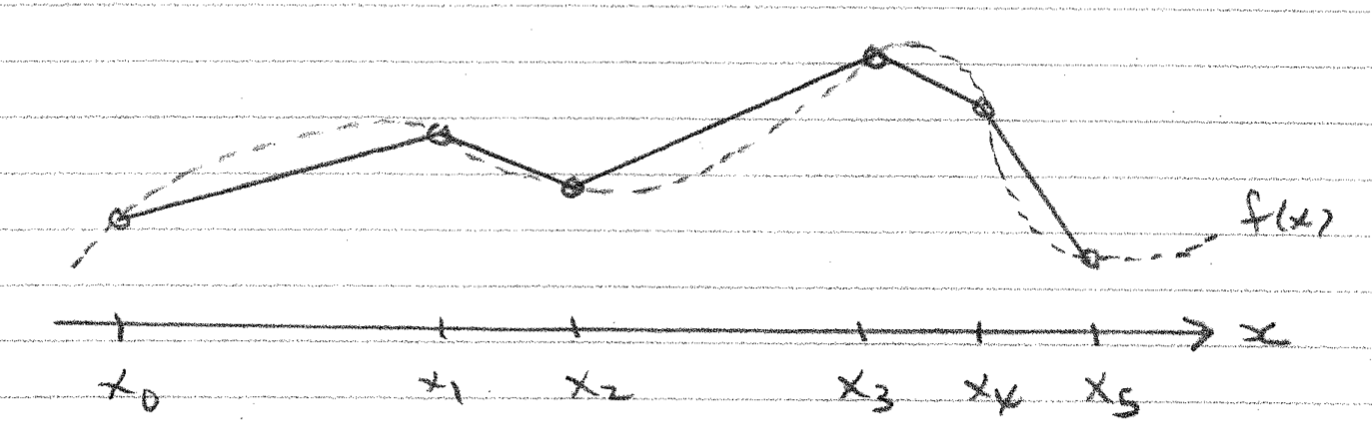
\includegraphics[scale=0.4]{linear_splines}
  \caption{Example of linear spline}
  \label{fig:linear}
\end{figure}


Disadvantage of piecewise linear polynomials: 
not differentiable (at points $x_i$, the knots). 
\end{frame} 

\begin{frame}{Quadratic splines}
Differentiability can be obtained by using quadratic (instead of linear) 
polynomials on each $[x_i, x_{i+1}]$. 


\begin{figure} 
  \centering
  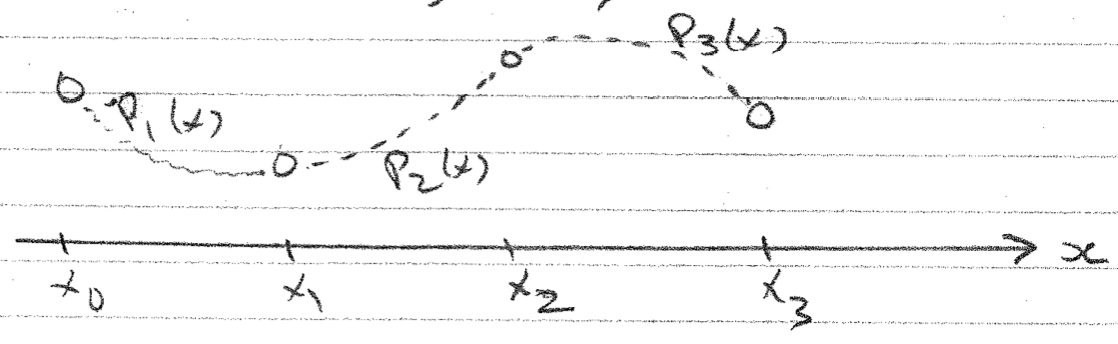
\includegraphics[scale=0.5]{quadratic_splines}
  \caption{Example of quadratic spline}
  \label{fig:quad}
\end{figure}
\end{frame} 


\begin{frame}{Quadratic splines} 
\begin{itemize}
\item Each $P_i(x)$ is a quadratic (and is not uniquely determined) 
\item The piecewise polynomial can be made differentiable on $[x_0, x_n]$ 
\item If differentiable, this is an example of a \underline{spline function} 
\end{itemize}  

\end{frame}  

\begin{frame}{Spline Defintion} 

{\bf Definition:} 
$S(x)$ is a spline function on $[x_0, x_n]$ if for some $q \geq 1$ 
\begin{enumerate} 
\item $S(x)$ is a polynomial of degree $q$ on each subinterval $[x_i, x_{i+1}]$ 
\item $S(x)$ and its first $q-1$ derivatives are continuous on $[x_0, x_n]$ 
\end{enumerate}
\vspace{\baselineskip}
{\bf Spline types:}
\begin{itemize} 
\item Linear spline, $q=1$
\item Quadratic spline, $q=2$
\item Cubic spline, $q=3$
\end{itemize} 
\end{frame}

\begin{frame}{Physical splines} 
\begin{figure} 
  \centering
  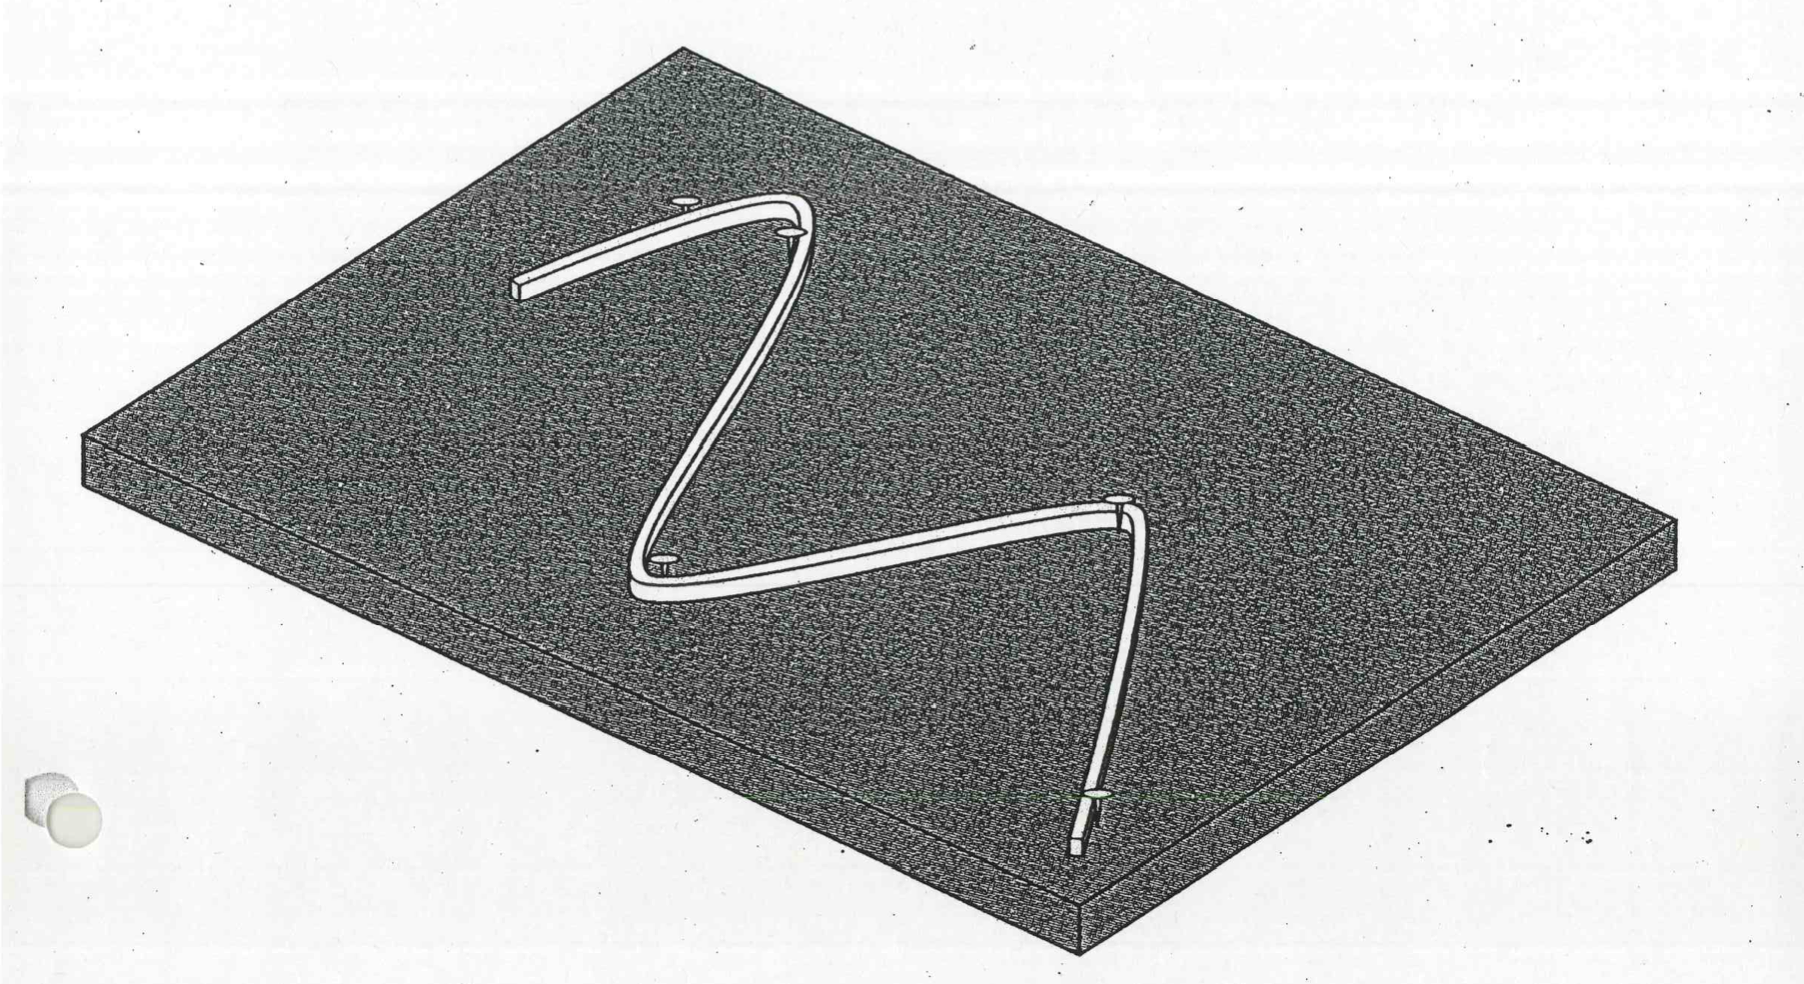
\includegraphics[scale=0.3]{physical_splines}
  \caption{Drafting technique of using a spline to draw smooth curves 
through a series of points}
  \label{fig:draft}
\end{figure}
\end{frame} 


\begin{frame}{History}
Splines were first defined by Schoenberg in 1946. Note that the definition of a spline function does {\bf not} require that it interpolates some given function $f(x)$. But splines are often used as interpolating functions (a spline interpolant): 
\begin{itemize} 
\item They do not have the osciallatory nature of high degree interpolating polynomials 
\item They require no derivatives of $f(x)$, except possibly at the end points $x_0$ and $x_n$. 
\end{itemize} 

The most common spline interpolant is {\bf cubic}. 
\end{frame} 

\begin{frame}{Applications}
\begin{itemize}
\item{Graphics} 
\begin{itemize} 
\item Smooth curves (continuity) 
\end{itemize}
\item{Animation}
\begin{itemize} 
\item Modeling = specifying shape 
\item Animation = specifying shape over time 
\item Real objects don't move in straight lines - \href{https://www.youtube.com/watch?v=gGbXldn522A}{Video}
\end{itemize}
\item{Motion Control}
\begin{itemize}
\item{embedded systems}
\item{automated motion}
\item{robotics}
\end{itemize}
\end{itemize} 
\end{frame} 

\section{Cubic Spline Interpolants}

\begin{frame}{Cubic Spline Interpolants}

{\bf Definition:} Given $x_0,x_1,...,x_n$ with $x_i < x_{i+1}$ for each $i$, and $f(x_0), f(x_1), ..., f(x_n)$, then $S(x)$ is a {\bf cubic spline interpolant} for $f(x)$ if,

\begin{enumerate}[(a)]
\item{$S(x)$ is a cubic polynomial, denoted by $S_j(x)$, on each subinterval $[x_j,x_{j+1}]$, for $j=0,...,n-1$}
\item{$S_j(x_j)=f(x_j)$, for $j=0,...,n-1$ and $S_{n-1}(x_n)=f(x_n)$}
\item{$S_{j+1}(x_{j+1})=S_j(x_{j+1})$, for $j=0,...,n-2$}
\item{$S'_{j+1}(x_{j+1})=S'_j(x_{j+1})$, for $j=0,...,n-2$}
\item{$S''_{j+1}(x_{j+1})=S''_j(x_{j+1})$, for $j=0,...,n-2$}
\item{either one of the following hold:}
\begin{enumerate}[(i)]
\item{$S''(x_0)=S''(x_n)=0$ (natural bounds), or}
\item{$S'(x_0)=f'(x_0)$ and $S'(x_n)=f'(x_n)$ (clamped bounds)}
\end{enumerate}
\end{enumerate}

\end{frame}

\begin{frame}{Cubic Spline Interpolants II}

{\bf Notes:}
\begin{itemize}
\item{for any $f(x)$, there exist an infinite number of cubic splines satisfying conditions (a) - (e). Why?}
\item{There are $n$ cubic polynomials $S_j(x)$ to specify, each one is defined by 4 coefficients, giving a total of $4n$ unknowns to be specified.}
\item{However, condition (b) gives $n+1$ conditions to be satisfied, and (c), (d) and (e) each give $n-1$ conditions to be satisfied.}
\item{Thus, there are $(n+1)+3(n-1)=4n-2$ conditions (equations) to be satisfied in $4n$ unknowns.}
\item{But if either (i) or (ii) is also required to be satisfied, then there are $4n$ conditions in $4n$ unknowns and there exists a \underline{unique} cubic spline interpolant satisfying (a) - (f).}
\end{itemize}
\end{frame}

\begin{frame}{Example 1 - Cubic Spline}
Determine $a_0,b_0,d_0,a_1,b_1,c_1,$ and $d_1$ so that
\[
S(x) = \left\{
\begin{array}{ll}
     a_0+b_0x-3x^2+d_0x^3, & -1 \leq x\leq 0 \\
     a_1+b_1x+c_1x^2+d_1x^3, & 0 \leq x\leq 1 
\end{array}
\right. \]
is the natural cubic spline function such that $S(-1)=1, S(0)=2,S(1)=-1$.
\vspace{2 in}
\end{frame}

\begin{frame}{Example 1 continued}

\end{frame}

\begin{frame}{Example 1 continued}

\end{frame}

\begin{frame}{Cubic Splines in MATLAB}
There is an algorithm for spline computation given in the text but it has a different derivation than what we have done and different from MATLAB. In MATLAB they use a different form for the splines. For example, when $n=3$, MATLAB uses the following form for the cubic polynomials:
\begin{align*}
     S_0(x) &= a_0+b_0(x-x_0)+c_0(x-x_0)^2+d_0(x-x_0)^3 \\
     S_1(x) &= a_1+b_1(x-x_1)+c_1(x-x_1)^2+d_1(x-x_1)^3 \\
     S_2(x) &= a_2+b_2(x-x_2)+c_2(x-x_2)^2+d_2(x-x_2)^3
\end{align*}


Note that, with this form, $a_0=f(x_0), a_1=f(x_1),$ and $a_2=f(x_2)$. This simplifies the system somewhat.

\end{frame}

\begin{frame}{Quadratic Spline}
Construction of quadratic splines is similar to that of cubic splines but there are only $3n$ unknown coefficients and you do not need to set the second derivatives of the interior knots to be equal. That is, we do not create the (e) equations from above. As such, the (b) to (d) equations total $3n-1$, meaning that we also only need one extra (f) equation. Often we use $Q''(x_0)=0$ or, as is the case with the next example, we assign one of the coefficients before hand.
\end{frame}

\begin{frame}{Example 2 - Quadratic Spline}
Determine $a,b,c,d,$ and $e$ so that
\[
Q(x) = \left\{
\begin{array}{ll}
      ax^2+x+b, & -1 \leq x\leq 0 \\
     cx^2+dx+e, & 0 \leq x\leq 1 
\end{array}
\right. \]
is a quadratic spline function that interpolates $f(x)$ where $f(-1)=1, f(0)=1,f(1)=1$.
\vspace{2 in}
\end{frame}

\begin{frame}{Example 2 continued}

\end{frame}

\end{document} 



